%%%%%%%%%%%%%%%%%%%%%%%%%%%%%%%% 
\section{The Data Acquisition System (DAQ) and Computing}
\label{cdrsec:detectors-nd-ref-daq-comp}

The scope of the Near Detector System DAQ and computing includes the design, procurement, fabrication, testing, delivery and installation of all the systems and components that comprise it: \fixme{complete this intro}


\subsection{NDS DAQ}
\label{cdrsec:nd-gdaq-intro}

The Near Detector System (NDS) Data Acquisition system (NDS-DAQ) collects raw data from each NDS 
detector's individual DAQ, issues triggers, adds precision timing 
data from a global positioning system (GPS), and builds events. 
The NDS-DAQ is made up of three parts, as shown in the block diagram of 
Figure~\ref{fig:DAQ_Block}, a master DAQ and one each for the near neutrino detector (NND, which is the FGT) and the BLM systems. The names for these are, respectively, NDS-MDAQ, NND-DAQ and BLM-DAQ.

\begin{cdrfigure}[Near Detector System DAQ block diagram]{DAQ_Block}{Near Detector System DAQ block diagram: The NDS-DAQ consists 
of the NDS Master DAQ (green blocks), the Beamline Measurement DAQ (yellow summary 
block) and the Near Neutrino Detectors DAQ (orange summary block).  The 
NDS-DAQ connects to other portions of DUNE and LBNF, shown here in other colors (blue, 
light red, tan).}
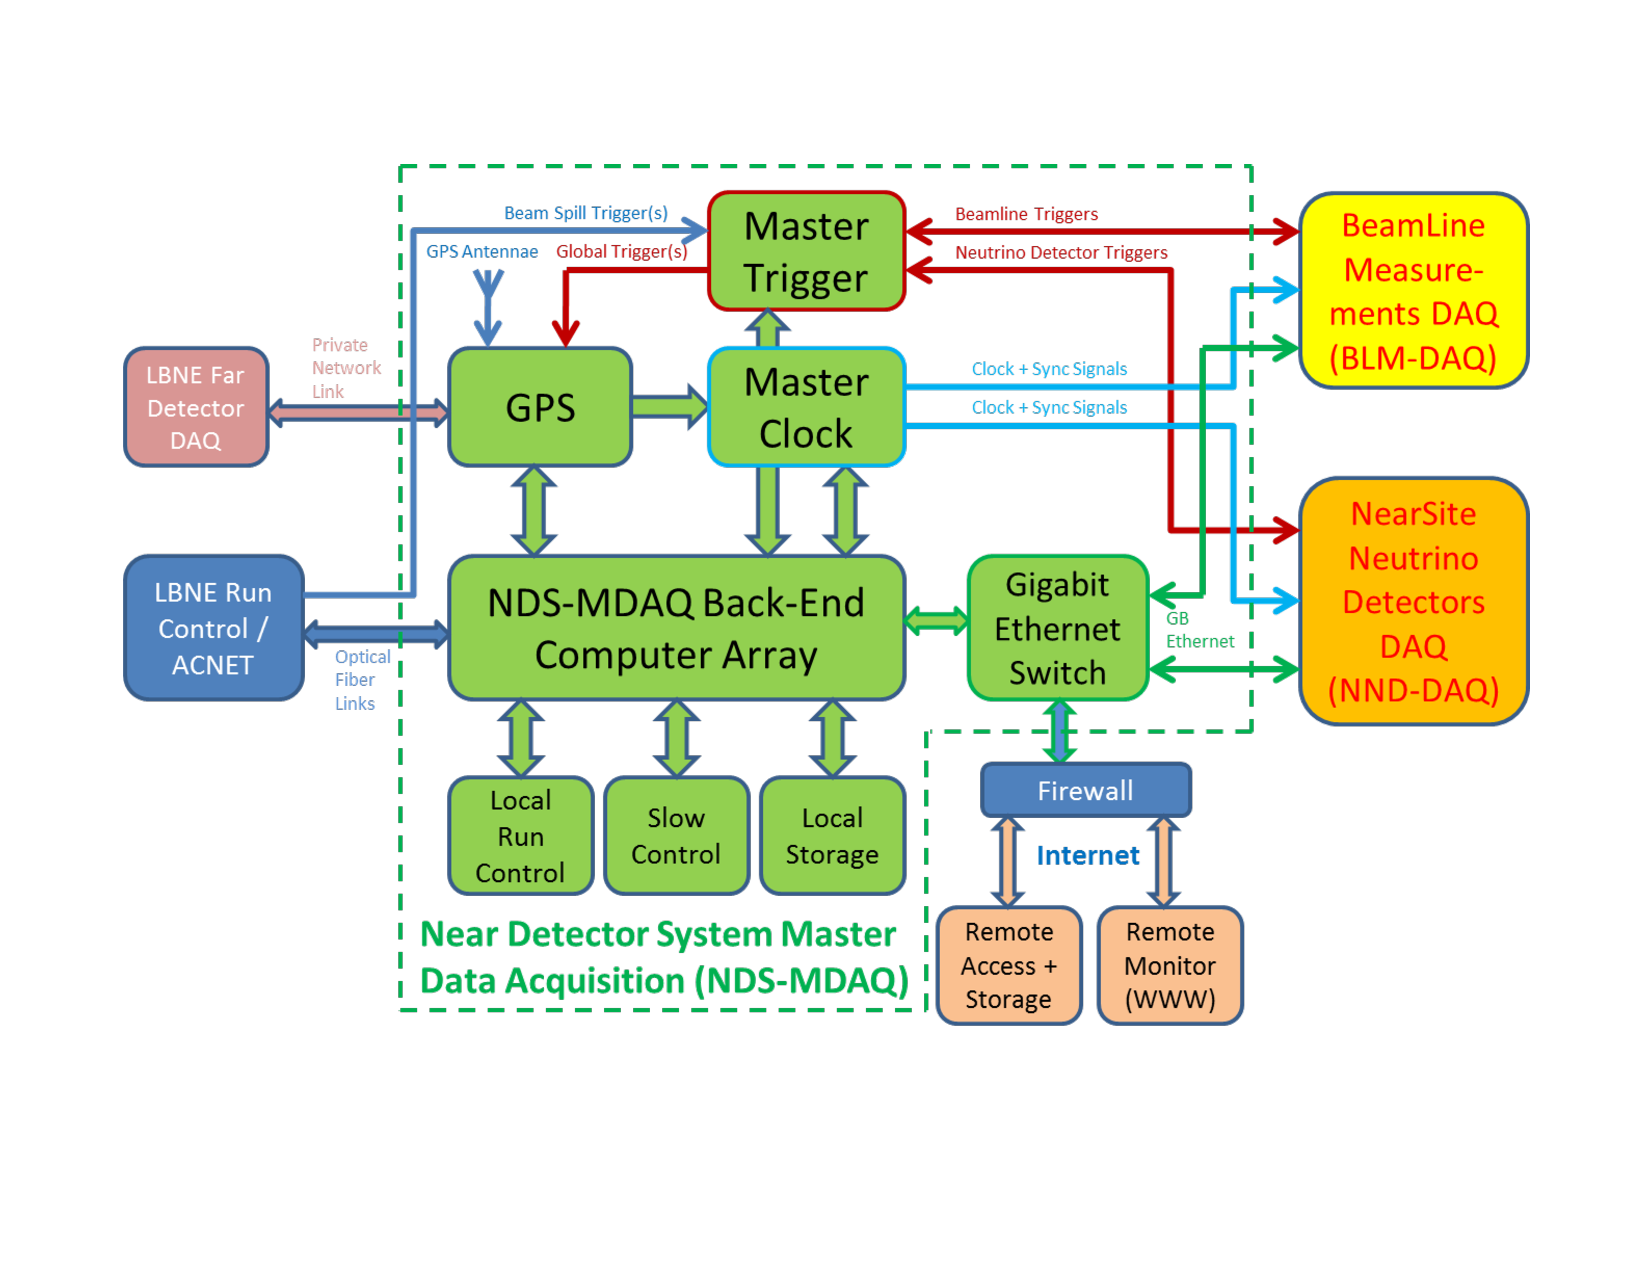
\includegraphics[width=6in,angle=0]{DAQ_Block}
\end{cdrfigure}

\subsubsection{NDS Master DAQ} 
\label{cdrsec:nd-master-daq}

The NDS Master DAQ (NDS-MDAQ) is designed to provide a high-level user interface 
for local run control and data taking, as well as for secure remote control and monitoring.   It will 
serve as the primary interface to the NND-DAQ and BLM-DAQ and will include the following:
\begin{itemize}
\item slow-control system 
\item online data and DAQ performance monitoring  
\item raw data collection
\item building of events
\item data storage.   
\end{itemize}
The NDS-MDAQ includes hardware two-way triggering for both the NND-DAQ and BLM-DAQ, and 
GPS hardware for precision time-stamping and global clock synchronization. 
The design is currently based on a channel count estimate of approximately 433,000 
from the near neutrino detector, plus $<1,000$ 
from the beamline detectors.  Custom electronic components for the NDS-DAQ are based on existing 
custom designs from other experiments, e.g., T2K and ATLAS, and 
implement commercial components for the trigger modules, clock and timing synchronization, 
GPS and environmental monitoring.


\subsubsection{Near Neutrino Detector DAQ (NND-DAQ)} 
\label{cdrsec:nd:nnd:daq}


The Near Neutrino Detector Data Acquisition system (NND-DAQ) collects raw data from 
the DAQ in each NND subdetector and connects to the 
NDS Master DAQ via Gigabit Ethernet. A block diagram of the NND-DAQ is
shown in Figure~\ref{fig:DAQ_NND}. The NND-DAQ will mainly consist 
of a scalable back-end computer array, interconnected to the individual 
subdetector DAQs via Gigabit Ethernet, and specialized electronics modules for trigger 
processing and clock synchronization. It interfaces to the NDS-MDAQ for 
run control and data collection. The NND-DAQ will also have its own local run-control setup, 
consisting of a number of desktop workstations to allow independent local runs that include 
NND subdetectors only; this is useful during detector commissioning, calibration runs, 
stand-alone cosmic runs, or other runs where the beam is stopped or not needed.

The quantity of computers required for the NND-DAQ back-end system is highly dependent on the 
number of channels and expected data rates of the individual neutrino detectors. 
One back-end computer should be able to handle 
approximately 3,000 channels for sustainable and continuous runs. Assuming a total of 
433,000 channels for all NND subdetectors combined, about 150 back-end computers would be 
needed.

Trigger signals from each subdetector will be collected and pre-processed by a 
trigger electronics module, similar in design to the NDS  trigger or master-clock modules 
of the NDS-MDAQ design. Depending on the run mode, this module could feed local 
trigger 
decisions to the detector DAQs for data collection, or it could forward NDS triggers 
from the NDS-MDAQ or higher levels to the NND subdetector DAQs.  A slave-clock electronics 
module, similar to the master-clock module in the NDS-MDAQ, distributes clock- and 
time-synchronization signals from the NDS-MDAQ to all NND subdetectors.


\begin{cdrfigure}[A block diagram of the Near Neutrino Detector DAQ]{DAQ_NND}{A block diagram of the Near Neutrino Detector DAQ (NND-DAQ).}
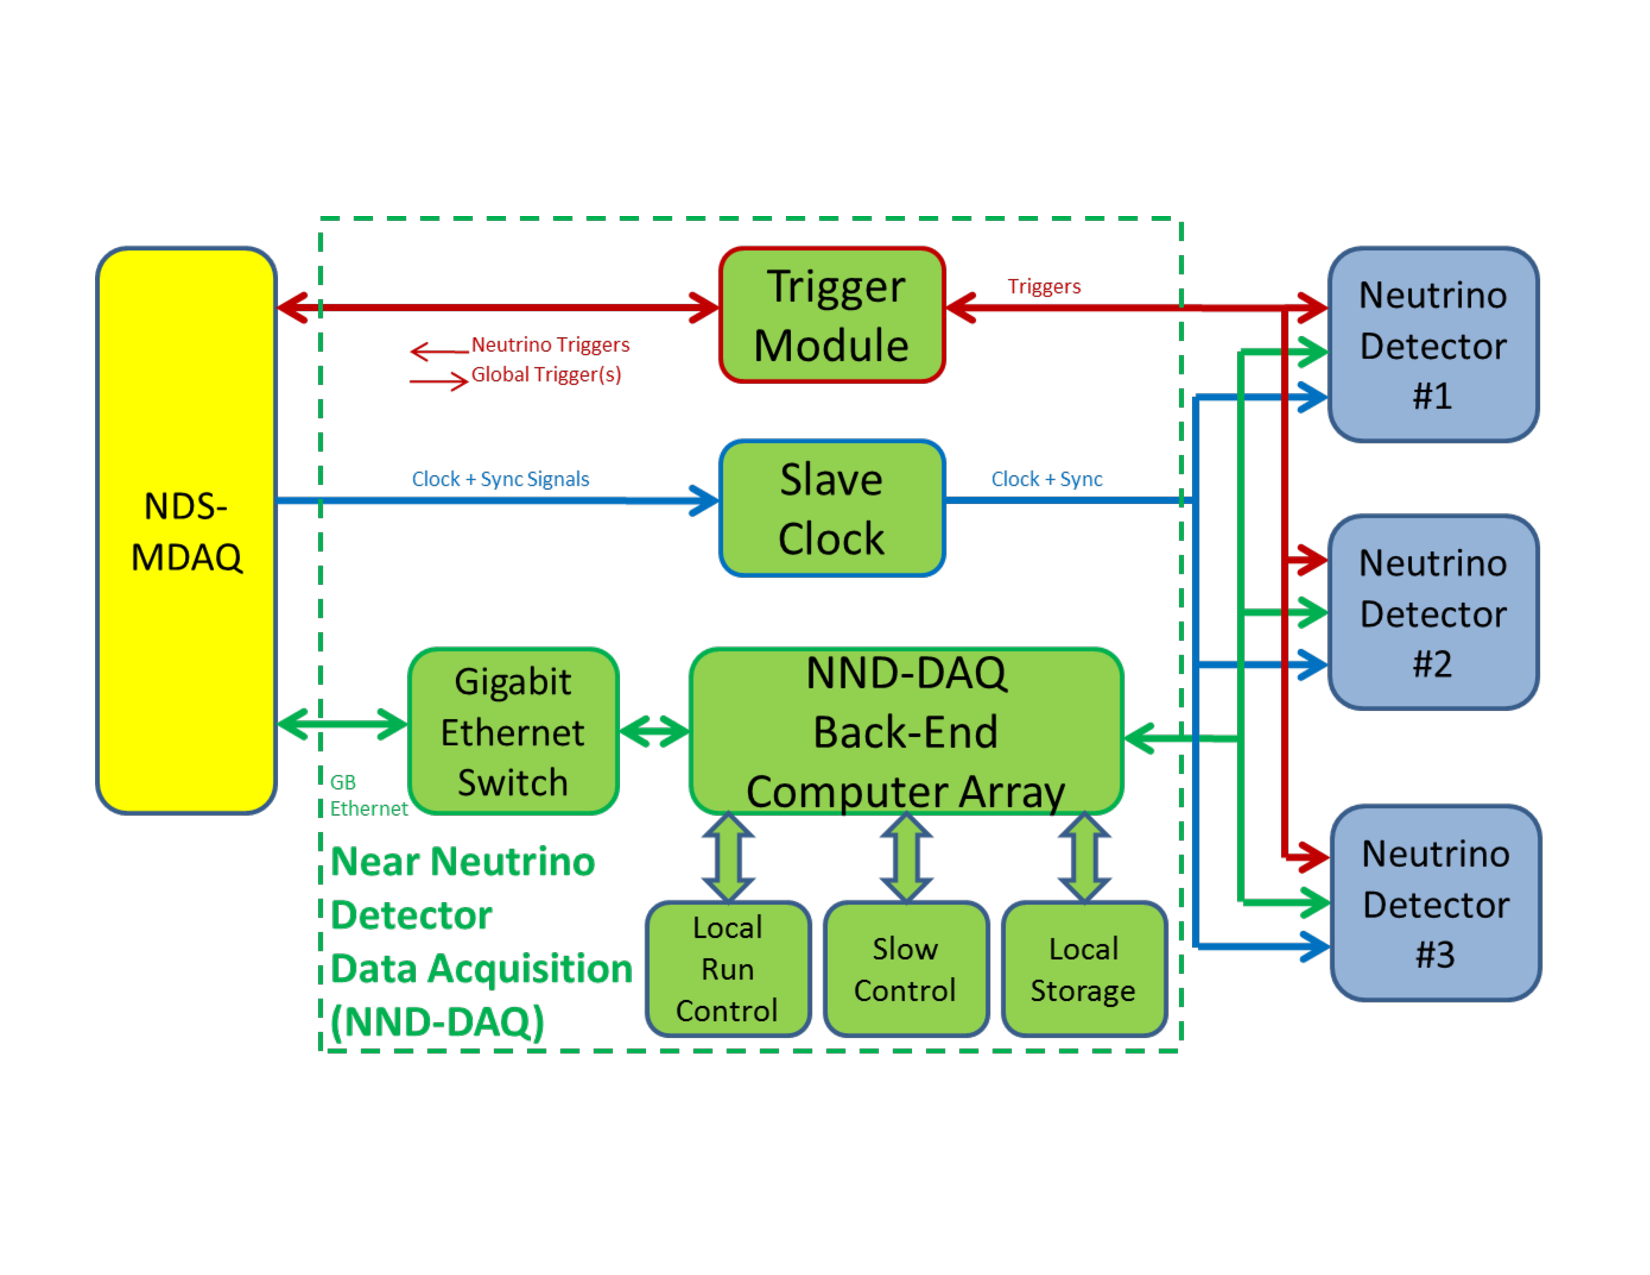
\includegraphics[width=6in,angle=0]{DAQ_NND}
\end{cdrfigure}


\subsubsection{Beamline Measurements DAQ (BLM-DAQ)}

The BLM-DAQ will mainly consist of a scalable back-end 
computer array, inter-connected to the individual beamline measurement detector DAQs via 
Gigabit Ethernet and specialized electronics modules for trigger processing and clock 
synchronization. It interfaces to the NDS-MDAQ for run control and 
data collection. It will also have its own local run-control setup, consisting of a number 
of desktop workstations to allow independent local runs that include beamline measurement 
detectors only; this is useful during detector commissioning, calibration runs, stand-alone cosmic 
runs or other runs where the beam is stopped or not needed.


\subsection{NDS Computing}
\label{cdrsec:nd-gdaq-global-computing}

The computing system encompasses two major activities: online computing with required 
slow-control systems, and offline computing for data analysis and event simulation.
The computing components are based 
on currently available commercial computing and gigabit networking technology, which is 
likely to improve over the next years without driving costs up for the final design.  

